\documentclass[11pt]{article}
\usepackage[utf8]{inputenc}
\usepackage[french]{babel}
\usepackage[T1]{fontenc}
\usepackage{verbatim}
\usepackage{graphicx}
\usepackage{fullpage}
\usepackage{hyperref}
\author{Contzen Laurent}

\begin{document}

\begin{titlepage}  
  \begin{flushleft}
    Contzen Laurent
  \end{flushleft}
  \begin{center}
    \vspace{85mm}\LARGE{\textbf{STIC-B-415 : Architecture des Systèmes d'Information.} \\    
      Les bases de données de type NoSQL.}
  \end{center}
  \begin{flushright}
    \vspace{95mm}
    Année Académique 2011-2012.             
  \end{flushright}
\end{titlepage}

\tableofcontents
\newpage
\vspace*{\fill}
\begin{flushright}
  A DBA walks into a bar and leaves immediatly. \\
  He couldn't find a table. \\
  \textit{- Anonymous}
\end{flushright}
\vspace*{\fill}
\newpage

\section{Introduction}
\textbf{\textbf{TODO}} : Faire attention à différencier bases de données et gestionnaires de bases de données \\
Opposées aux bases de données relationnelles, les bases de données de faisant partie de la mouvance NoSQL (Not only SQL) sont non relationnelles, distribuées, horizontalement scalable (\textbf{FIXME}) et open-source. Bien que le terme NoSQL ait été utilisé pour la première fois en 1998 par Carlo Strozzi pour nommer le DBMS \footnote{Database management system} relationnel qu'il venait de développer, la vraie naissance de cette mouvance eut lieu en 2009 lorsque Eric Evans utilisa ce terme dans une discussion sur les bases de données distribuées. Ces dernières devenant de plus en plus importantes dans le web actuel, il était logique de travailler sur le sujet quitte à remettre en question un modèle en place depuis plusieures décénies. \textbf{TODO} : Préciser quelque part dans l'intro que NoSQL est généralement interprété comme Not only SQL et pas No SQL.
\section{Historique}
Les bases de données ont toujours été quelque chose de fondamental en informatique. En effet, stocker de grandes quantité d'informations et pouvoir y accéder et les traiter rapidement et efficacement est un des buts fondamentaux de cette discipline. \\
Au départ, chaque système était lié à sa propre base de données, étudiée et optimisée pour lui. Ceci posait évidemment, comme beaucoup de choses à cette époque, de gros problèmes de portabilité de données et changer un système informatique avait d'énormes implications. Il était donc nécéssaire et urgent de standardiser ça, chose qui a été faite par le Database Task Group qui proposa en 1971 un standard qui fut connu en tant que ``Codasyl Approach''. Cette approche était navigationnelle et basée sur une navigation manuelle d'un ensemble d'informations disposées en ``réseau''. \\
C'est ensuite dans les années 1970 qu'un ingénieur travaillant chez IBM, Edgar Codd, révolutionna le monde des bases de données avec son article ``A Relational Model of Data for Large Shared Data Banks'' qui posa les fondations des bases de données relationnelles. Les principes énoncés dans cet articles furent implémentés, testés, et un langage de requêtes standardisé, le SQL, fit son apparition en même temps. \\
Les bases de données relationnelles utilisant SQL se sont très vite répandues et plusieures implémentations apparurent telles que DB2, Microsoft SQL Server, PostgreSQL, MySQL, etc. \\
C'est ensuite bien plus récemment, vers la fin des années 2000, que ce modèle a été remis en question et que plusieurs modèles de bases de données non relationnelles sont apparus.
\section{Le modèle relationnel}
Pour pouvoir comprendre les différences entre le modèle relationnel et la mouvance qui nous occupe ici, commençons par décrire ce modèle historique. \\
Dans une base de données relationnelle, les données sont organisées sous forme de tables. Dans ces tables, les colonnes sont les champs, et le contenu des lignes les données. Une ligne d'une table est donc un ensemble de données contenant les différents champs de la table pour une même entité \textbf{FIXME}. \textbf{TODO}: Préciser qu'un schéma doit être défini à l'avance. Par exemple, immaginons une table Characters contenant les informations sur des personnages de séries. Imaginons que les informations nécéssaires sur un personnage sont son ID, son nom, la série de laquelle il vient et l'acteur qui le jouait. La table Characters pourra être : \\
%% \begin{figure}[H]
%%   \centering
\begin{center}
  \begin{tabular}{| c | l | l | l | l |}
    \hline
    \textbf{\underline{Id}} & \textbf{Name} & \textbf{Show} & \textbf{Actor} \\
    \hline
    \hline
    1 & Jackson Teller & Sons of Anarchy & Charlie Hunnam \\
    \hline
    2 & John Dorian & Scrubs & Zach Braff  \\
    \hline
    3 & Bill Adama & Battlestar Galactica & Edward James Olmos \\
    \hline
    4 & Kara Thrace & Battlestar Galactica & Katee Sackhoff \\
    \hline
    5 & Tyrion Lannister & Game of Thrones & Peter Dinklage \\
    \hline
    6 & Ted Mosby & How I Met Your Mother & Josh Radnor \\
    \hline
    7 & Seth Bullock & Deadwood & Timothy Oliphant \\
    \hline
    8 & Tobias Beecher & Oz & Lee Tergesen \\
    \hline
    9 & Emily Sullivan & Jericho & Ashley Scott \\
    \hline
    10 & Jimmy McNulty & The Wire & Dominic West \\
    \hline
  \end{tabular}
\end{center} 
%%   \caption{Exemple de table Character dans une base de données relationnelle.}
%% \end{figure}
C'est ensuite le langage SQL qui sera utilisé pour faire des requêtes dans la base de données pour en extraire des informations. On parlera aussi d'effectuer une transaction. Une transaction est une action dans la base de données comme insérer une nouvelle entrée dans un table, mettre à jour un champ ou récupérer des informations. Par exemple, pour afficher tout le contenu de la table Characters on pourra faire : \\
\verb@SELECT * FROM Characters;@, \\
pour récupérer tous les personnages de la série Battlestar Galactica on pourra faire : \\
\verb@SELECT * FROM Characters WHERE Show = ``Battlestar Galactica'';@, \\
ou encore pour savoir qui a joué le rôle de Tyrion Lannister dans la série Game of Thrones : \\
\verb@SELECT Actor FROM Characters WHERE Name=''Tyrion Lannister'' AND Show=''Game of Thrones'';@. \\ 
\textbf{TODO} : Parler d'une partie des opérations possibles comme l'insertion, les jointures, etc.
Le langage SQL présenté ci dessus est un langage de requêtes standardisé et extrèment répandu, mais les bases de données relationnelles reposent aussi sur des fondements mathématiques théoriques tels que l'algèbre relationnelle. Tout ceci est extrèmement formalisé, ce qui peut être vu dans beaucoup de cas comme un point positif, et demande donc beaucoup de rigueur et une grande réflexion sur la structure de la base de données avant de commencer à la créer. Or, dans le cadre du Web de nos jours il est parfois extrèmement difficile de pouvoir prévoir à l'avance quel champs seront nécéssaires, quel type de données ils devront contenir, etc. \\
Deux autres grands problèmes des bases de données relationnelles sont la possibilité de redimmensionner facilement (scalability) et les moyens de distribuer dans divers data centers à travers le monde. \textbf{TODO} : Compléter ca \\
\textbf{TODO} : adapter le hardware à la volée, changer la structure d'une db, toussa. \\
\textbf{TODO} : Refaire l'ordre du texte pour présenter le SQL avant de montrer les exemples.

\section{ACID et CAP}
Les deux familles de bases de données qui nous occupent ici sont basées chacune sur des principes de base, respectivement ACID pour le modèle relationnel et CAP pour le modèle NoSQL. \\
\subsection{ACID}
ACID est un acronyme pour Atomicity, Consistency, Isolation, Durability. L'atomicité garantit qu'une transaction soit réussit, soit échoue. Il n'y a donc pas de statut intermédiaire, c'est à dire que si une transaction échoue l'entièreté des modifications apportées par celle ci devra être annulée. On ne pourra donc pas avoir une insertion qui échoue mais dont la moitié des champs est présente dans la base de données par exemple. \\
Le principe de consistance signifie que la base de données est dans un état ``correct'' avant et après chaque transaction. L'atomicité et la consistance sont donc deux principes intimement liés. \\
L'isolation quand à elle va forcer les transaction à être indépendantes les unes des autres, et si deux transactions doivent modifier une même donnée l'une des deux sera mise en attente jusqu'à ce que la pemière ait fini. \\
Enfin, la durabilité implique qu'une fois qu'une transaction est terminée les modifications apportées par cette dernière resteront dans la base de données, meme si celle-ci se vautre lamentablement comme un veau bouré. \\
Cet ensemble de principes assure donc que la base de données restera cohérente dans tous les cas et permet d'éviter au maximum les données corrompues. Mais tout ceci a un coût. Par exemple, si la base de données doit subir une très grande quantité de transactions en très peu de temps (par exemple, le nombre de tweets à la seconde sur twitter lors de gros évènements peut facilement submerger une base de données si le hardware est pas prévu pour supporter ca et pouvoir réagir extrèmement rapidement) le principe d'isolation va fortement ralentir le processus.
\subsection{CAP}
Le théorème CAP, aussi connu sous le nom de Brewer's theorem (du nom d'Eric Brewer qui l'a proposé en 2000 lors d'un symposium sur l'informatique distribuée), statue qu'il est impossible pour tout système de données partagées de garantir simultanément les trois principes suivants : consistance, disponibilité et tolérance à la partition/répartition (\textbf{FIXME}) (Consistency, Availability and Partition tolerance, CAP). \textbf{TODO}: Rajouter qu'il a été prouvé en 2002. \\
La terme consistance dans CAP n'est pas du tout à interpréter de la manière énoncée précédemment de ACID : dans ce cas-ci il représente le fait que lorsqu'une donnée est insérée ou modifiée, toute personne y accédant aura toujours la dernière version de l'information. \\
La disponibilité quand à elle représente le fait qu'on peut considérer que la db est toujours up et répondra en permanence au requêtes qui lui sont envoyées. Pour arriver à cet objectif les dbs seront répandues sur énormément de serveurs physiques agissant comme une seule base de données avec la puissance de tous les serveurs la composant. \\
Pour finir, la tolérance à la partition signifie que l'ensemble des données sera toujours accessible, même si une partie des serveurs est totalement innaccessible. Ceci permet surtout de répandre la db dans beaucoup de data centers (et si l'un tombe, les autres continuent de fournir les infos). Si une information doit être écrite dans un noeud temporairement innaccessible, elle sera écrite autre part puis quand le noeud reviendra up ce qu'il a raté lui sera transmis et il se mettra à jour. Sans ce type de mécanismes les dbs sont condamnées à devoir être dans un seul et unique data center. 
\section{Différents use-cases}
Comme le démontre la différence entre CAP et ACID, les bases de données relationnelles et les bases de données de type NoSQL ne suivent pas les mêmes idées et vont avoir des use cases différents. Tout ce qui touche au système bancaire (et aux transactions financières, à l'argent, ...) devra avoir la certitude que les données sont consistantes (au sens ACID du terme) et qu'aucune donnée ne sera jamais perdue. On peut aussi considérer que les changements de structures de bases de données dans ce large domaine sont assez rares, et qu'il n'y a pas un grand besoin d'élasticité niveau offre de ressources due à des pics d'utilisation. Les bases de données NoSQL ne sont donc absolument pas adaptées (en tous cas à ce jour) à ce type de domaine. \\
Par contre, les réseaux sociaux sont un excellent exemple de situations dans lesquelles les bases de données NoSQL sont bien plus adaptées que leur ancêtre historique (\textbf{FIXME}). En effet, la quantité de données circulant dessus est astronomique (et en constante expension) mais très irrégulière, et si un staut facebook mets quelques minutes à apparaitre dans la timeline d'une relation à l'autre bout du monde (le temps de répliquer l'information à travers les data centers) ce n'est absolument pas grave. De plus, la scalability (\textbf{FIXME}) des serveurs est quelque chose de crucial. Avoir en permanence des serveurs capables de tenir les pics de charge les plus rares couterait une fortune, et ces serveurs seraient presque tout le temps largement sous utilisés. Pouvoir modifier la capacité du système pour absorber un pic et puis revenir à la situation précédente permet donc d'effectuer de grandes économies, économies sans lesquelles certaines entreprises ne pourraient pas survivre. Par exemple, les MTV Video Music Awards ont engendré 8868 tweets par seconde sur twitter le 28 aout 2011, alors qu'en temps normal le nombre de tweets par seconde est extrèmement inférieur à celà. Devoir maintenir des serveurs pouvant tenir cette charge là en permanence signifierait probablement la mort de twitter. \textbf{TODO} : Reformuler tout l'aspect financier et préciser que les banques ont les moyens de se payers des RDBMSs qui tiennent la route. \\
\textbf{TODO} : parler de reddit qui mixe les deux

\section{Les grandes familles} % \textbf{TODO} : famille? autre terme?
La mouvance NoSQL est composée d'un ensemble de DBMSs qui partagent donc beaucoup d'aspects philosophiques (\textbf{FIXME}) et techniques mais les techniques d'implémentations varient beaucoup. On peut identifier plusieurs familles principales partageant aussi l'aspect technique du type d'implémentation. \textbf{FIXME} : formulation pourrie. \\
\textbf{TODO} : Dans chaque subsection mentionner des exemples ``connus'' et les dévelloper en deux mots si possible/nécéssaire. Préciser aussi que chaque DBMSs NoSQL a ses langages de requests.
\begin{center}
  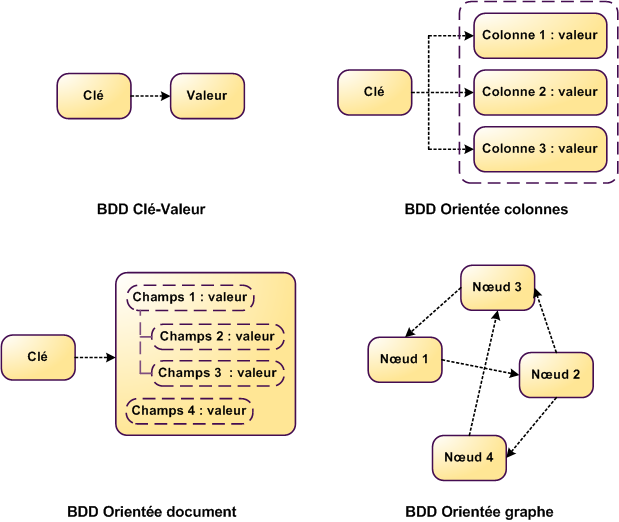
\includegraphics[width=12cm]{nosql.png}
\end{center}
\subsection{Les bases de données de type Key-Value}
Les bases de données de type Key-Value (clé-valeur) peuvent être vues comme de très grandes tables de hashage. L'idée de base est que dans certaines applications la plupart des accès à la base de données ne sont que des lectures ou écriture à partir d'un indentifiant. Dans ce cas, il n'est pas nécéssaire d'avoir toute la puissance du SQL et, surtout, de devoir subir la lourdeur qui y est associée puisque la plupart des possiblités du SQL ne seront jamais utilisées. Dans le cas des Key-Value, la base de données considère la valeur comme un bloc binaire sans savoir ce qu'il contient et ne sais donc faire aucune opération dessus si cela s'avèrait nécéssaire. \\
Techniquement, les données seront insérées dans une table partitionnée utilisant un mécanisme de hashage consistant, ce qui permet de répartir uniformément la charge et la quantité de données entre les différentes tables. Ensuite, les données seront répliquées sur d'autres machines, pouvant contenir chacune plusieurs partitions afin de limiter le nombre minimum d'instances de réplication nécéssaires. Il reste alors la consistance à garantir. Pour avoir une consistance parfaite, il serait nécéssaire de s'assurer qu'à chaque changement dans une table cette modification est bien répliquée dans toutes les instances contenant cette partition mais ceci a évidement un coût niveau efficacité. On va alors définir un taux de consistance souhaité, et s'assurer que au minimum ce pourcentage là des instances est mis à jour. Un mécanisme similaire sera mis en place pour assurer la consistance lors des écritures. Ceci permet de perdre un peu de la certitude de la consistance des données mais d'optimiser l'efficacité du service. \\
\textbf{TODO} : Schémas
\subsection{Les bases de données orientées document}
Cette famille de DBMSs est une extension du modèle Key-Value. Dans ce cas-ci, l'idée de base est le fait que souvent les pages web renseignent un ensemble d'informations ayant un lien clair (par exemple un même utilisateur) mais qui devraient être stockées dans beaucoup de tables différentes dans une structure relationnelle, ce qui serait très coûteux en jointures logiques. Dans une base de données orientée document nous avons, tout comme dans une db key-value, une clé pour accéder aux données, mais au lieu d'avoir un bloc binaire comme données c'est un document structuré (un peu comme un document XML) et le DBMS a connaissance du contenu du document, ce qui permet d'effectuer des opérations sur ces données sans toutes fois avoir autant de possibilités (et à nouveau de lourdeur) qu'avec SQL. \\
L'implémentation d'une base de données orientée document sera sensiblement la même que celle d'une base de données de type key-value mais il lui sera rajouté la ``conscience'' des données qu'elle contient ainsi que des mécanismes de traitements spécifiques à ces données (requêtes plus élaborées, accès à une partie des données seulement sans devoir charger l'entièreté des données associées à la clé, modifications de certains champs seulements, etc). C'est donc en quelque sorte un mélange entre les deux philosophies. \\
Cette famille, dont le but est de prendre le meilleur des deux mouvances, permettra par exemple de stocker une grande quantité d'informations qui aurait été plus limitée dans le modèle relationnel parfois trop rigide.
\subsection{Les bases de données orientées colonnes}
Les bases de données orientées colonnes sont elles aussi une extension du type key-value et un mélange avec des principes du modèle relationnel. Dans ce cas, la clé donne accès à un ensemble d'informations structurées en colonnes contenant des informations. Les données sont donc structurées mais cette structure présente des avantages non néglieables par rapport aux RDBMSs classiques lorsque la base de données contient énormément d'informations. \\
\begin{center}
  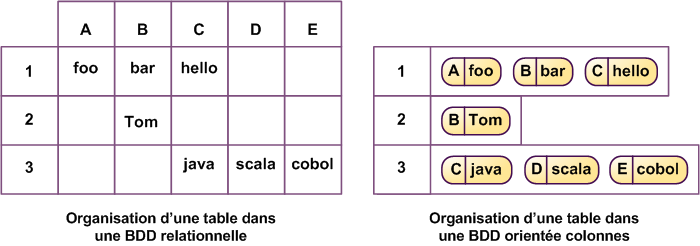
\includegraphics[width=12cm]{nosql-colonnes.png}
\end{center}
Tout d'abord, lorsqu'une colonne ne contient pas d'informations pour une clé, la colonne n'existe simplement pas pour elle, ce qui amène à un gain d'espace disque considérable lorsque la base de données contient (ou plutot devrait contenir en modèle relationnel) plusieurs millions de colonnes. Ensuite, l'ajout de colonnes se faisant à la volée et uniquement pour les entités concernées, l'adaptation de la structure aux nouveaux besoins ou aux changements de design ou de code est immédiate et ne demande aucun effort particulier. Ce modèle permet aussi de faire des requêtes simples sur les données, bien plus simples que leur équivalent SQL. \\
Apache Cassandra, une base de données orientées colonnes développée par Facebook, étends encore ce modèle en proposant la possibilité de faire des méta-colonnes, c'est à dire de contenir des colonnes dans des colonnes. Cela permet une meilleure organisation des données, et, surtout, une optimisation des requêtes vu que l'ensemble de colonnes à considérer n'est qu'un sous-ensemble précis défini à l'avance.
\subsection{Les bases de données orientées graphe}
Les bases de données orientées graphe sont quant à elles en rupture avec les autres catégories de la mouvance NoSQL. En effet, elles sont basées sur la théorie des graphes et ne partagent pas beaucoup de points techniques avec les autres. Les données seront donc organisées en noeuds, arcs et propriétés. \\
\begin{center}
  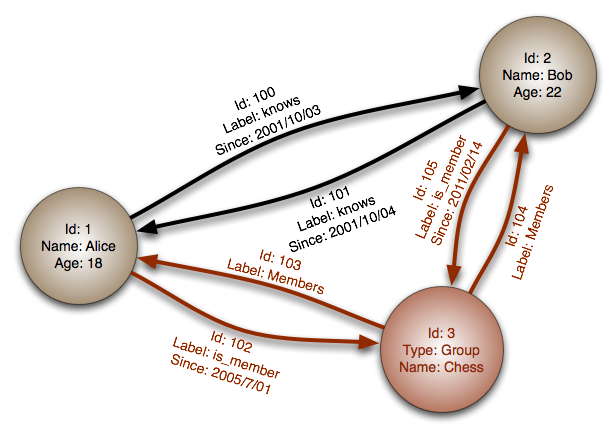
\includegraphics[width=12cm]{nosql_graph.png}
\end{center}
Les noeuds, que l'on pourrait comparer à des objets dans de la programmation orientée objet, représentent ici des entités auxquelles sont associées des propriétés et les arcs qui les relient représentent les relations existant entre ces entités et fournissent des informations à leurs propos. Ceci apporte une flexibilité absolue puisqu'il n'y a pas besoin d'établir un schéma de la structure : chaque noeud ou arc peut-être rajouté n'importe quand et contenir n'importe quelle information désirée. Pour les cas où avoir un schéma peut être utile, voire nécéssaire, il est tout de même possible d'en définir un qui sera après utilisé pour garantir une cohérence (\textbf{FIXME}) entre les noeuds. La théorie des graphes et ses applications étant très utilisée en informatique, il existe déjà des algorithmes très poussés pour le parcours et la recherche par exemple. \\
Les bases de données orientées graphes permettent d'obtenir certaines opérations extrèmement simplement. Par exemple, le réseau social professionnel LinkedIn établit le niveau de séparation entre deux personnes simplement en calculant la distance entre les noeuds concernés.
\subsection{Les autres bases de données}

\section{Conclusion}
Nous voyons donc que la plupart des modèles de la mouvance NoSQL ne rejette pas en bloc l'ensemble des idées des RDBMSs mais en prélève plutôt une partie à laquelle ils essayent d'ajouter de la souplesse, de la perfomance afin de, tout simplement, avoir une solution plus optimisée aux besoins. \textbf{FIXME} : formulation pourrie.
\section*{Sources}
\url{http://www.thoughtworks.com/articles/nosql-comparison} \\
\url{http://www.linuxjournal.com/article/10770} \\
\url{http://nosql-databases.org/} \\
\url{http://nosql-database.org/links.html} \\
\url{http://en.wikipedia.org/wiki/NoSQL} \\
\url{http://en.wikipedia.org/wiki/Dbms} \\
\url{http://en.wikipedia.org/wiki/NoSQL_(RDBMS)} \\
\url{http://stackoverflow.com/questions/3596461/is-there-any-good-book-on-nosql} \\
\url{http://www.computerworld.com/s/article/9135086/No_to_SQL_Anti_database_movement_gains_steam_} \\
\url{http://blog.xebia.fr/2010/04/21/nosql-europe-tour-dhorizon-des-bases-de-donnees-nosql/} \\
\url{http://www.techrepublic.com/blog/10things/10-things-you-should-know-about-nosql-databases/1772} \\

\end{document}
